%~~~~~~~~~~~~~~~~~~~~~~~~~~~~~~~~~~%
%   PIERO CAMPALANI                %
%   Curriculum-vitae               %
%~~~~~~~~~~~~~~~~~~~~~~~~~~~~~~~~~~%

% workarond for bibentry/hyperref compatibility issues
% http://www.tug.org/applications/hyperref/ftp/README
\makeatletter
\let\saved@bibitem\@bibitem
\makeatother
% --------- %

\pdfminorversion=4
\documentclass[10pt]{article}
\usepackage[margin=3cm]{geometry}
\usepackage{marvosym}		% mobile phone symbol
\usepackage{textcomp}		% born symbol
\usepackage{fixltx2e}		% text subscript
\usepackage{titling}		% vspace title/author
\posttitle{\par\end{center}}
\usepackage{fancybox, graphicx}
\usepackage{longtable}		% tables across pages
\setlength{\LTpre}{0pt}
\setlength{\LTpost}{0pt}
\usepackage{bibentry}
\usepackage{hyperref}		% hyperlinks
\graphicspath{{./pics/}{/usr/share/doc/texlive-doc/latex/minitoc/}}	% countries flags
\DeclareGraphicsExtensions{.pdf,.png,.jpg}
\DeclareMathAlphabet{\mathpzc}{OT1}{pzc}{m}{it}	% mathzpc style

% New definitions
% For RGB hexs, see: http://www.html.am/html-codes/color/color-code-chart.cfm
\usepackage[table,usenames,dvipsnames]{xcolor}
\definecolor{grey}{gray}{0.2}
\definecolor{medgrey}{gray}{0.5}
\definecolor{lightgray}{gray}{0.8}
\definecolor{verylightgray}{gray}{0.95}
\definecolor{palegoldenrot}{HTML}{EEE8AA}
\definecolor{lightgoldenrodyellow}{HTML}{FAFAD2}
\definecolor{lightslategrey}{HTML}{778899}
\newcolumntype{L}{>{\raggedleft}p{0.14\textwidth}}
\newcolumntype{R}{p{0.8\textwidth}}
\newcommand\VRule{\color{lightgray}\vrule width 0.7pt}

\usepackage{colortbl}

% hyperref defaults
% http://stackoverflow.com/questions/544907/remove-boxes-from-hyperlinked-toc-in-latex
\hypersetup{%
    pdfborder = {0 0 0}
}


% TITLE ~~~~~~~~~~~~~~~~~~~~~~~~~~~~~~~~~~~~~~~~~~~~~~~~~~
\title{\bfseries\Huge Piero Campalani}
%\author{\emph{curriculum vitae}\thanks{Last update: \today.}} -- puts a line in the second page..
\author{\emph{curriculum vitae}\textsuperscript{*}}
\date{}

\pagenumbering{roman}

\begin{document}
\maketitle
\let\thefootnote\relax\footnote{\textsuperscript{*}Last update: \today.}

% PERSONAL INFO ~~~~~~~~~~~~~~~~~~~~~~~~~~~~~~~~~~~~~~~~~~
\vspace{-.5cm}
\begin{minipage}[ht]{0.2\textwidth}
\raggedright
  \shadowbox{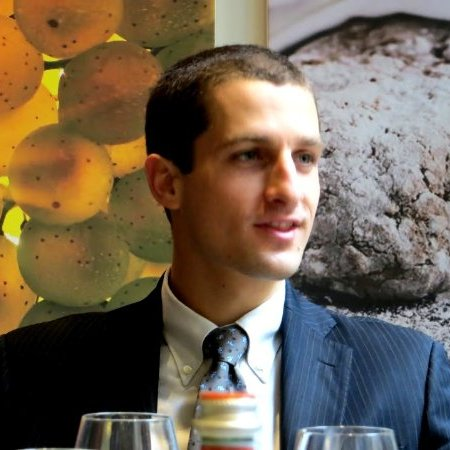
\includegraphics[width=2.2cm]{avatar}}
\end{minipage}
\begin{minipage}[ht]{0.33\textwidth}
  \begin{flushleft}
  \begin{tabular}{ c l }
    \textborn & 1985 Noviembre 1\textsuperscript{st}\\
              & Portomaggiore (FE), IT\\
    \Mobilefone & 
\includegraphics[width=3mm]{italy-f} $\mathpzc{{\scriptstyle +}39\,333\,412\,83\,17}$\\
                & 
\includegraphics[width=3mm]{spain-f} $\mathpzc{{\scriptstyle +}34\,611\,209\,861}$
  \end{tabular}
  \end{flushleft}
\end{minipage}
\begin{minipage}[ht]{0.33\textwidth}
  \begin{flushright}
  \begin{tabular}{ c l }
    \Letter & Via della Resistenza n.18\\
           & 44121 Ferrara, IT\\
    {\small \MVAt} & \href{mailto:piero.campa@gmail.com}{\texttt{piero.campa@gmail.com}}\\[3pt]
    
\includegraphics[width=3.5mm]{earth-logo} &
                    \href{https://www.ohloh.net/accounts/pierocampa}{
\includegraphics[width=4mm]{ohloh-logo}}
                    \href{https://www.researchgate.net/profile/Piero_Campalani/}{
\includegraphics[width=4mm]{researchgate-logo}}
                    \href{https://www.linkedin.com/pub/piero-campalani/19/4a6/b13}{
\includegraphics[width=4mm]{linkedin-logo}}
                    \href{https://careers.stackoverflow.com/users/info/189094}{\includegraphics[width=4mm]{{careers2.0-logo}.pdf}}
  \end{tabular}
  \end{flushright}
\end{minipage}
\vspace{.5cm}

% SUMMARY ~~~~~~~~~~~~~~~~~~~~~~~~~~~~~~~~~~~~~~~~~~~~~~~~
\section*{Presentaci\'on}
\small
Investigador motivado y comprometido, me encanta hacer frente a los nuevos desaf\'ios y la implementaci\'on. 
En mi experiencia en \textbf{\mbox{\emph{geo}-inform\'atica}}, me desenvuelvo mejor dentro de entornos de colaboraci\'on de c\'odigo abierto. 
Creo en la importancia de los debates abiertos y peopleware, en el an\'alisis y dise\~no (y en los comentarios de c\'odigo) preventivo.

Despu\'es de graduarme como \emph{ingeniero} de TLC en la Universidad de Ferrara, 
gan\'e experiencia como analista espacial para aplicaciones de calidad del aire durante mi doctorado, 
el desarrollo de modelos geoestad\'isticos multivariable para la estimaci\'on de la
exposici\'on de part\'iculas, con las im\'agenes de sat\'elite.

Despu\'es de terminar el \emph{doctorado}, he trabajado en la Universidad Jacobs de Bremen durante 
2 a\~nos y 6 meses, dise\~nando e implementando servicios web de geo-imagenes del OGC (WCS\slash WCPS)
para la visualizaci\'on y procesamiento de conjuntos de datos cuadriculados espacio-temporales
a trav\'es del proyecto \mbox{open-source} \texttt{rasdaman}.
~\\ ~\\
En los \'ultimos a\~nos he trabajado mucho en \textbf{ambientes internacionales} junto a los 
miembros de mi equipo, supervisando a los estudiantes y proporcionando apoyo continuo a la 
comunidad \mbox{\textbf{open-source}} dispuesta a utilizar nuestro software.

He presentado mi investigaci\'on en diversas conferencias cient\'ificas internacionales.
Soy capaz de resumir los aspectos clave de mi trabajo y presentarlo a los dem\'as en 
diferentes contextos: desde la breve presentaci\'on para principiantes hasta tutoriales
t\'ecnicos para workshop espec\'ificos.

T\'ecnicamente, manejo bien Linux desde hace a\~nos y muchos lenguajes de programaci\'on 
(por ejemplo, Java, Bash, R, o C\slash C++); me he encargado de dise\~no e implementaci\'on de bases 
de datos PostgreSQL activos; soy un entusiasta de \textsl{git}, y puedo lidiar f\'acilmente con el 
desarrollo distribuido y versionado.
Por \'ultimo, cuando se trata de mostrar resultados, prefiero trabajar con Inkscape, Gimp y \LaTeX{}.

% OCCUPATIONAL FIELD ~~~~~~~~~~~~~~~~~~~~~~~~~~~~~~~~~~~~~
\section*{Campos Laborales Deseados}
{\normalsize An\'alisis\slash Modelos Espaciales $\cdots$ Teledetecci\'on $\cdots$ Ciencia de los Ordenadores $\cdots$ Telecomunicaciones.}

\pagebreak
% PROFESSIONAL EXPERIENCE ~~~~~~~~~~~~~~~~~~~~~~~~~~~~~~~~
\section*{Experiencia Profesional}
\begin{longtable}{L!{\VRule}R}
\rowcolor{SpringGreen}
2015--\emph{now}& \textbf{Development Engineer} en Ebotlution Systems S.L., Barcelona, España.\\
              & \footnotesize\textit{Ingeniería de soluciones innovadoras para la remoción de minas en el campo del Desminado Humanitario: 
              detecci\'on automatica de minas/UXO a trav\'es de droides, monitoreo por telemetr\'ia en tiempo real, 
              multi-actor protocol de red, avanzada interfaz de usuario SIG con los sistemas de soporte de decisiones} --- 
              la iniciativa es un proyecto de I\&D.\\[5pt]
\rowcolor{verylightgray}
2013--2014 & \textbf{PostDoc} en el grupo de investigaci\'on Large-Scale Scientific Information Systems (LSIS) en Jacobs University Bremen, Alemania.\\
             & \footnotesize\textit{Dise\~no y desarrollo para el acceso y el an\'alisis via Web de series temporales regulares e irregulares
               de imagenes satelitales \mbox{geo-referenciadas} a trav\'es de la base de datos \textnormal{\texttt{rasdaman}} y su servlet Java. 
               Participaci\'on activa en el grupo OGC ``Temporal Ad-Hoc'' para la definici\'on de sistemas de coordenadas \mbox{espacio-temporales}}
               --- beca de investigaci\'on EU~FP7 para el proyecto ``EarthServer''.\\[5pt]
\rowcolor{verylightgray}
2012--2013   & \textbf{PhD visitante} en el grupo de investigaci\'on Large-Scale Scientific Information Systems (LSIS) en Jacobs University Bremen, Alemania.\\
             & \footnotesize\textit{12 meses de investigaci\'on y desarrollo sobre la base de datos \textnormal{\texttt{rasdaman}} y su interfaz Web
               para el acceso online de imagenes georeferenciadas. Equipo de investigaci\'on internacional, desarrollo software FOSS de colaboraci\'on,
               dise\~no e implementaci\'on de servicios OGC (WCS, WCPS, WMS)} --- beca de investigaci\'on EU~FP7 para el proyecto ``EarthServer''.\\[5pt]
%$\Downarrow$ &\\[5pt]
\rowcolor{verylightgray}
2010--2012   & \textbf{PhD de pr\'acticas} en MEEO Srl, Ferrara, Italia.\\
             & \footnotesize\textit{23 meses de investigaci\'on sobre la valoraci\'on de imagenes satelitales MODIS de aerosol
               para la creaci\'on de mapas de exposici\'on PM\textsubscript{10}. Construcci\'on de modelos kriging multivariables con \textnormal{\texttt{R}},
               validaci\'on de mapas satelitales via fot\'ometros AERONET e implementaci\'on de interfaz Web GIS para la visualizaci\'on de
               datasets de calidad del aire a tierra, de modelo y de satelite.} --- beca de investigaci\'on de desarrollo regional para el proyecto
               ``SENSing, mOdeling and distRibution of EnviRonmental data (SENSORER)''.
\end{longtable}

% EDUCATION ~~~~~~~~~~~~~~~~~~~~~~~~~~~~~~~~~~~~~~~~~~~~~~
\vspace{.5cm}
\section*{Formaci\'on}
\begin{longtable}[t]{L!{\VRule}R}
\rowcolor{SkyBlue}
2010--2012& \textbf{PhD} en \textsl{Ciencias de la Ingenier\'ia} en la Universidad de Ferrara, Italia.\\[-2pt]
          & \footnotesize\emph{Titulo tesis:} Geostatistical modelling of PM$_{10}$ mass concentrations with satellite imagery from MODIS sensor\\[-2pt]
          & \footnotesize\emph{Nota final:} Ottimo\\[-2pt]
          & \footnotesize\emph{Ciclo de doctorado:} XXV\\[-2pt]
          & \footnotesize\emph{Duraci\'on:} 3 a\~nos\\[7pt]
\rowcolor{verylightgray}
      2009& Habilitaci\'on profesional (\textbf{Esame di Stato}) como \textsl{Ingeniero de la Informaci\'on} en la Universidad de Bolonia, Italia.\\[-2pt]
          & \footnotesize\emph{Categor\'ia:} Nuovo Ordinamento, secci\'on A\\[-2pt]
          & \footnotesize\emph{Nota final:} 211\slash 240\\[7pt]
\rowcolor{verylightgray}
2007--2009& \textbf{MSc} en \textsl{Ingenier\'ia Electr\'onica y de las Telecomunicaciones} en la Universidad de Ferrara, Italia.\\[-2pt]
          & \footnotesize\emph{Titulo tesis:} Architectures and Perfomance for Network Coding\\[-2pt]
          & \footnotesize\emph{Nota final:} 110\slash 110 cum laude\\[-2pt]
          & \footnotesize\emph{Duraci\'on:} 2 a\~nos\\[7pt]
\rowcolor{verylightgray}
2004--2007& \textbf{BSc} in \textsl{Ingenier\'ia Electr\'onica y de las Telecomunicaciones} en la Universidad de Ferrara, Italia.\\[-2pt]
          & \footnotesize\emph{Titulo tesis:} Robust Hash for Audio Identification\\[-2pt]
          & \footnotesize\emph{Nota final:} 109\slash 110 \\[-2pt]
          & \footnotesize\emph{Duraci\'on:} 3 a\~nos \\[7pt]
\rowcolor{verylightgray}
1999--2004& Diploma Cientifico de Escuela Superior en Liceo Scientifico A. Roiti, Ferrara, Italia.\\[-2pt]
          & \footnotesize\emph{Nota final:} 88\slash 100
\end{longtable}


% TRAINING COURSES ~~~~~~~~~~~~~~~~~~~~~~~~~~~~~~~~~~~~~~~
\pagebreak
\vspace{.5cm}
\section*{Cursos}
\begin{longtable}{L!{\VRule}R}
\rowcolor{palegoldenrot}
2017 & Curso de verano \textbf{Geo-computation using free and open source software} en la Universidad de Basilicata in Matera, Italia.\\[-2pt]
     & \footnotesize\emph{Description:} R, Grass, Python, Gdal/Ogr library y Linux.\\[-2pt]
     & \footnotesize\emph{Duration:} 5 d\'ias\\[7pt]
\rowcolor{lightgoldenrodyellow}
2014 & Curso de verano \textbf{Monitoring of the Earth System} en ESA\slash ESRIN, Italia.\\[-2pt]
     & \footnotesize\emph{Descripci\'on:} \textsc{Sistemas de Observaci\'on Globales}: Capacidades y aplicaciones de observaci\'on de la Tierra,
la f\'isica de la medici\'on de teledetecci\'on, el concepto de los sistemas de observaci\'on integrados de sistemas.
\textsc{Modelado del Sistema Tierra}: Principios b\'asicos del oc\'eano, la atm\'osfera, el terreno y el modelado de hielo, 
predicci\'on num\'erica del tiempo, predicci\'on por conjuntos.
\textsc{Asimilaci\'on de Datos}: Teor\'ia de las t\'ecnicas de asimilaci\'on de datos (por ejemplo, la interpolaci\'on \'optima, m\'etodos variacionales,
Filtro de Kalman, filtrado de conjunto) y las aplicaciones (por ejemplo, \mbox{re-an\'alisis}, modelaci\'on inversa, estimaci\'on de estado,
la teor\'ia del control, dise\~no de sistemas de observaci\'on \'optima, como definir las observaciones).
\textsc{Cambio Global}: Observaci\'on del cambio global desde el espacio, el uso del modelo de Sistema de la Tierra 
para comprender, predecir y gestionar las cuestiones ambientales.\\[-2pt]
     & \footnotesize\emph{Duraci\'on:} 10 d\'ias\\[7pt]
\rowcolor{palegoldenrot}
2013 & Curso de verano \textbf{Basic Aerosol Science} en la Facultad de Fisica de la Universidad de Viena, Austria.\\[-2pt]
     & \footnotesize\emph{Descripci\'on:} Introducci\'on a la mec\'anica de aerosoles; interacci\'on de la luz con las part\'iculas;
fen\'omenos de nucleaci\'on y de condensaci\'on; medici\'on de aerosol el\'ectrico; difusi\'on y filtraci\'on de part\'iculas;
qu\'imica fundamental del sistema de aerosol; qu\'imica sobre medici\'on en l\'inea;
espectroscopia moderna como una herramienta para la caracterizaci\'on de aerosol;
interacci\'on de las part\'iculas de aerosol con el pulm\'on: deposici\'on, eliminaci\'on y retenci\'on; partículas biol\'ogicas primarias;
medici\'on \'optica de part\'iculas; visibilidad y \'optica atmosf\'erica; separadores inerciales;
teledetecci\'on de aerosoles atmosf\'ericos; monitorizaci\'on y an\'alisis de datos.\\[-2pt]
     & \footnotesize\emph{Duraci\'on:} 10 d\'ias\\[7pt]
\rowcolor{lightgoldenrodyellow}
2012 & Curso de verano \textbf{GEOSTAT} en el Instituto de Geoinform\'atica de la Universidad de M\"unster, Alemania.\\[-2pt]
     & \footnotesize\emph{Descripci\'on:} An\'alisis de datos espaciales y espacio-temporal en \texttt{R}; \texttt{R} como SIG;
visualizaci\'on de datos \mbox{espacio-temporales} de \texttt{R} en Google Earth, tutoriales GRASS~GIS y SAGA~GIS;
agregaci\'on espacial y el cambio de soporte en la geoestad\'istica; geoestad\'istica espacio-temporal.\\[-2pt]
     & \footnotesize\emph{Duraci\'on:} 6 d\'ias\\[7pt]
\rowcolor{palegoldenrot}
2011 & Curso intensivo para estudiantes de doctorado \textbf{Analysing Spatial Data} por el Prof.~Roger Bivand en
       la Norwegian School of Economics (NHH), Bergen, Noruega.\\[-2pt]
     & \footnotesize\emph{Descripci\'on:} Introducci\'on a \texttt{R}, representaci\'on de datos espaciales en t\'erminos conceptuales y pr\'acticos;
visualizaci\'on \mbox{non-espacial} y el an\'alisis de datos espaciales; el an\'alisis de patrones de puntos; interpolaci\'on y geoestad\'istica;
datos de \'areas y de la econometr\'ia espacial; preparaci\'on de supervisi\'on y presentaci\'on  de proyecto.\\[-2pt]
     & \footnotesize\emph{Duraci\'on:} 8 d\'ias\\[7pt]
\end{longtable}

\pagebreak
% WORKSHOPS  ~~~~~~~~~~~~~~~~~~~~~~~~~~~~~~~~~~~~~~~
\definecolor{MidnightBlue}{RGB}{25,25,112} % http://cloford.com/resources/colours/500col.htm
\vspace{.5cm}
\section*{\underline{P}resentaciones\slash \underline{W}orkshops}
\begin{longtable}{L!{\VRule}R}
2014/07 & \textcolor{OrangeRed}{\scriptsize{[W]}}
          \textcolor{MidnightBlue}{\textit{``Spatio-Temporal Big Data --- the} rasdaman \textit{approach''}}\\[-2pt]
        & \textsc{OSGeo's European Conference on Free and Open Source Software for Geospatial} (Bremen, DE).\\[2pt]
2014/06 & \textcolor{Orange}{\scriptsize{[P--KEYNOTE]}}\textcolor{MidnightBlue}{\textit{``Server-side Maps Processing
          for the Air Quality with the WCPS Standard''}}\\[-2pt]
        & \textsc{International Workshop on Air Quality in Asia} (Hanoi, VN).\\[2pt]
        & \textcolor{OrangeRed}{\scriptsize{[W]}}
          \textcolor{MidnightBlue}{\textit{``Spatio-Temporal Big Data --- the} rasdaman \textit{approach''}}\\[-2pt]
        & \textsc{Open Source Geospatial Research and Education Symposium} (Espoo, FI).\\[2pt]
2014/04 & \textcolor{Orange}{\scriptsize{[P]}}
          \textcolor{MidnightBlue}{\textit{``EarthServer: Agile Analytics on Big Earth Data''}}\\[-2pt]
        & \textsc{Ecosystem approach to marine data workshop} (Athens, GR).\\[2pt]
2014/03 & \textcolor{Orange}{\scriptsize{[P]}}
          \textcolor{MidnightBlue}{\textit{``A Proposal for Temporal and Index CRSs for OGC-NA''}}\\[2pt]
        & \textsc{OGC Technical Committee Meeting} (Crystal City, VA, USA).\\[2pt]
2013/06 & Asistencia a \textsc{Big Data From Space} (ESA\slash ESRIN, IT)\\[2pt]
2013/03 & \textcolor{Orange}{\scriptsize{[P]}}
          \textcolor{MidnightBlue}{\textit{``Multi-Dimensional Space \& Time Support by Coordinate Reference Systems''}}\\[-2pt]
        & \textsc{OGC Technical Committee Meeting} (Abu Dhabi, UAE).\\[-2pt]
\end{longtable}

% LANGUAGES ~~~~~~~~~~~~~~~~~~~~~~~~~~~~~~~~~~~~~~~~~~~~~~
\vspace{.5cm}
\section*{Idiomas}
\begin{longtable}{L!{\VRule}R}
Italiano & Lengua materna\\[3pt]
Ingl\'es & Usuario independiente avanzado\\[-2pt]&\scriptsize\emph{12\slash 2010 Certificaci\'on Cambridge FCE (nivel B2 CEFR) -- Nota A}\\[3pt]
Espa\~nol & Usuario independiente avanzado\\[-2pt]&\scriptsize\emph{05\slash 2013 Certificaci\'on DELE (nivel B2 CEFR)}\\[3pt]
Alem\'an  & Usuario b\'asico
\end{longtable}

% MAIN SKILLS ~~~~~~~~~~~~~~~~~~~~~~~~~~~~~~~~~~~~~~~~~~~~
\vspace{.5cm}
\section*{Competencias}
\begin{longtable}{L!{\VRule}R}
\emph{Campos} & An\'alisis espacial y geoestadistica\\[-2pt]
              & Sistemas de navegaci\'on aut\'onoma\\[-2pt]
              & Servicios Web OGC (WCS\slash WCPS)\\[5pt]
\emph{T\'ecnico} & Aplicaci\'ones GIS\\[-2pt]
                 & Gesti\'on de database\\[-2pt]
                 & Desarrollo software de colaboraci\'on\\[-2pt]
                 & Comunicaciones radio\\[-2pt]
                 & Filtros de Kalmann\\[5pt]
\emph{Programaci\'on} & Java, C{}\verb!++!, R, bash, psql, PL\slash pgSQL, C, C\#, MATLAB, Python.\\[5pt]
\emph{Software} & Eclipse\slash NetBeans IDE, git, PostgreSQL, GDAL, OpenLayers, MapProxy, MapServer, PostGIS, \LaTeX.\\[5pt]
\emph{OS}       & Linux (Ubuntu), Windows.
\end{longtable}

\pagebreak
% BIBLIOGRAPHY ~~~~~~~~~~~~~~~~~~~~~~~~~~~~~~~~~~~~~~~~~~~
\vspace{.5cm}
\bibliographystyle{abbrv}
%\nobibliography{mybibliography}
% hyperref-bibentry compatibility workaround
\begingroup
  \makeatletter
  \let\@bibitem\saved@bibitem
  \nobibliography{mybibliography}
\endgroup
% -------- %
\section*{Publicaciones}
\begin{longtable}{L!{\VRule}R}
\textbf{2014} & \bibentry{campalani2014atmosphere}.\\[5pt]
              & \bibentry{yu2014gis}.\\[5pt]
              & \textcolor{lightslategrey}{\bibentry{yu2014point}.}\\[10pt]
\textbf{2013} & \bibentry{campalani2013integration}.\\[5pt]
              & \bibentry{campalani2013referenceable}.\\[5pt]
              & \bibentry{campalani2013spatiotemporal}.\\[5pt]
              & \textcolor{lightslategrey}{\bibentry{oosthoek2013towards}.}\\[5pt]
              & \textcolor{lightslategrey}{\bibentry{oosthoek2013innovative}.}\\[10pt]
\textbf{2012} & \bibentry{baumann2012finding}.\\[5pt]
              & \bibentry{campalani2012prediction}.\\[5pt]
              & \textcolor{lightslategrey}{\bibentry{nguyen2012aerosol}.}\\[10pt]
\textbf{2011} & \bibentry{campalani2011prediction}.\\[5pt]
              & \bibentry{campalani2011validation}.\\[5pt]
              & \textcolor{lightslategrey}{\bibentry{natali2011mea-pm}.}\\[10pt]
\textbf{2010} & \textcolor{lightslategrey}{\bibentry{nguyen2010aerosol}.}\\[5pt]
              & \bibentry{sensorer0154}.\\[5pt]
              & \bibentry{sensorer0153}.\\[5pt]
              & \bibentry{sensorer0152}.\\
\end{longtable}

% signature
\vspace{1.5cm}
\begin{figure}[h]
  \raggedleft
  
\includegraphics[width=40mm]{firma}
\end{figure}

\end{document}
